\documentclass[letterpaper]{scrartcl}
\usepackage[latin1]{inputenc}
\usepackage[T1]{fontenc}
\usepackage{textcomp}
\usepackage{mathptmx}
\usepackage[scaled=.92]{helvet}
\usepackage{courier}
\renewcommand*{\familydefault}{phv}
\usepackage[left=.5in,top=.5in,bottom=.5in,right=.5in]{geometry}
%\usepackage{fancyhdr}
%\lhead{UC Davis Biosport}\chead{}\rhead{Yeadon}
%\lfoot{}\cfoot{}\rfoot{}
%\pagestyle{fancy}
\usepackage{graphicx}
\usepackage{caption}
\usepackage{verbatim}
\usepackage{color}
\usepackage[
  pdftex,letterpaper=true,colorlinks=true,
  pdftitle={Key form},pdfsubject={Key},
  pdfauthor={ich},pdfpagemode=UseNone,pdfstartview=FitH,
  pagebackref,pdfhighlight={/N}
]{hyperref}
\begin{document}

\begin{center}
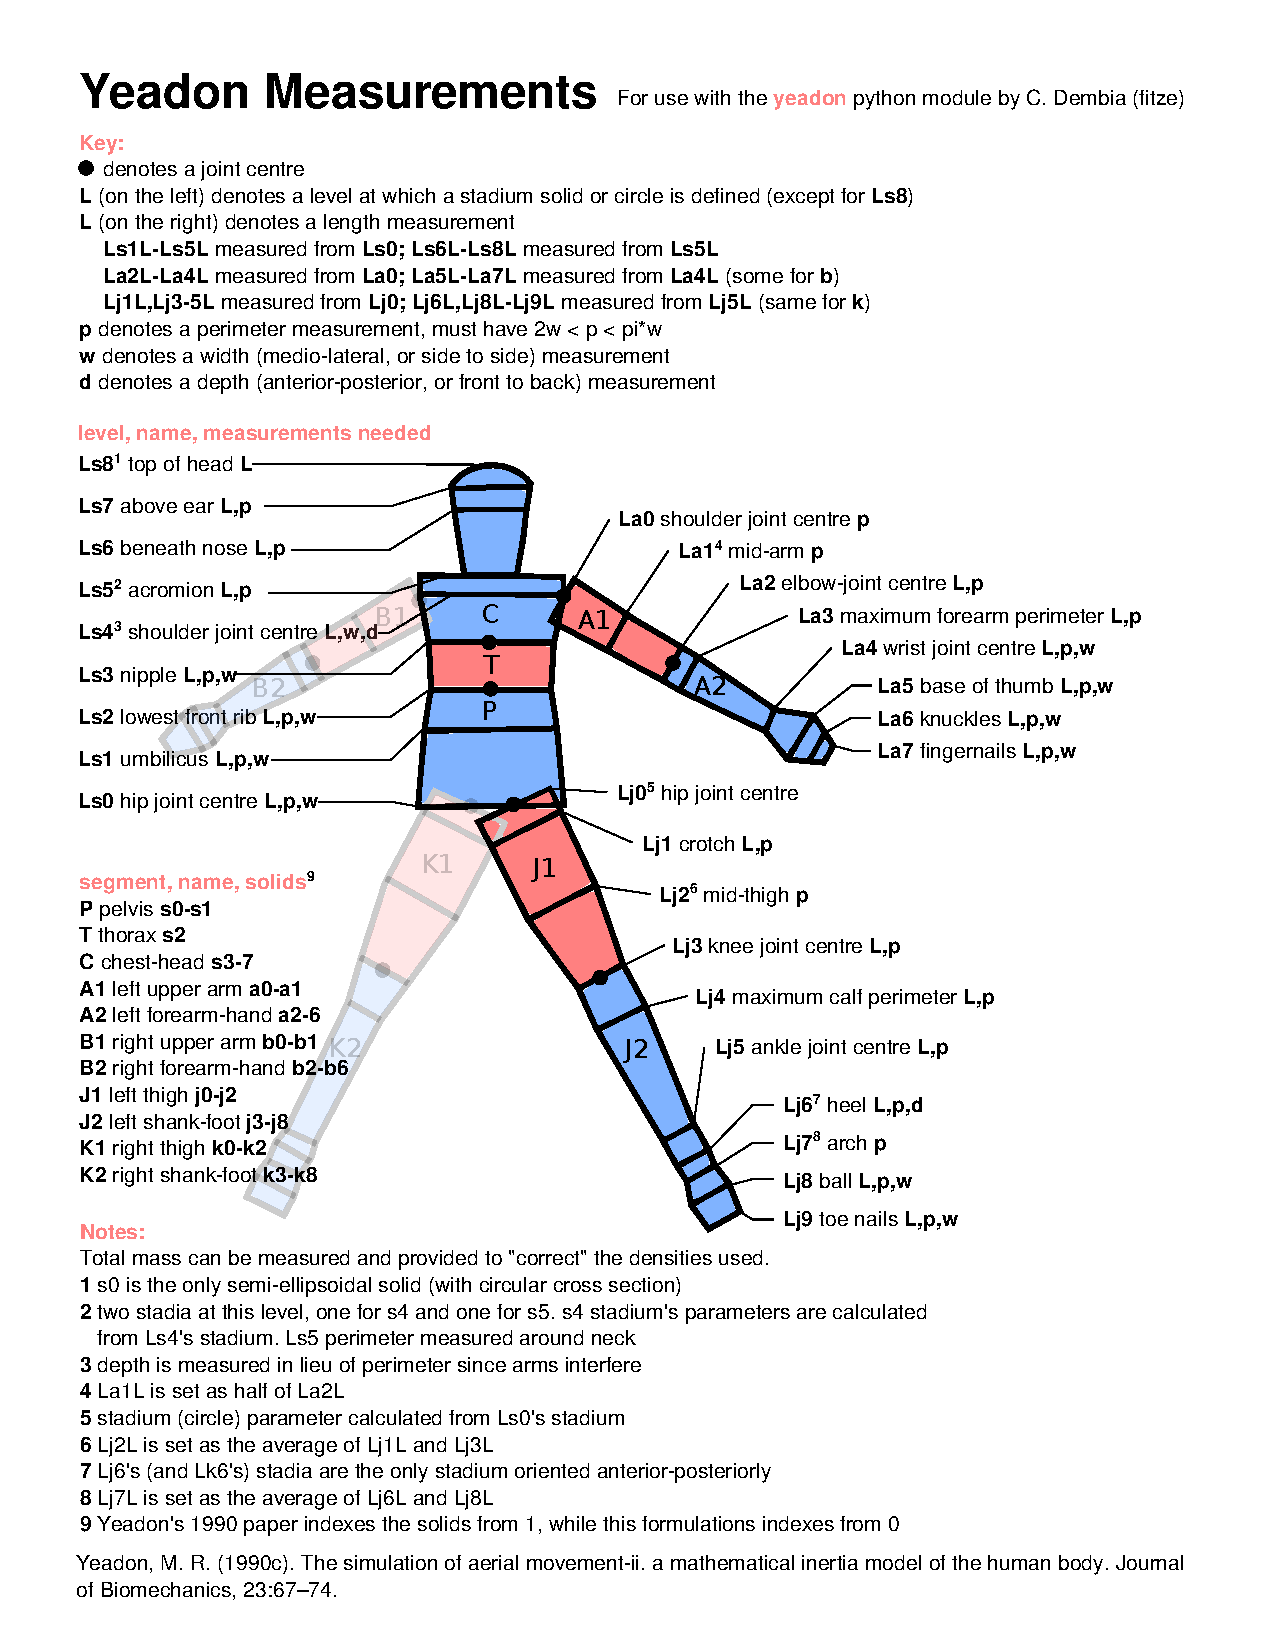
\includegraphics[width=170mm]{cld72_yeadon_meas_0716.pdf}
\end{center}

\newpage

\begin{Form}
\subsection*{Unit conversion}
Name: \TextField[name=Name,width=3in]{}  Date: \TextField[name=Date,width=2in]{}\\

measToMeters (number to convert from measurement units into meters): \TextField[name=measurementconversionfactor,width=.75in]{}
\subsection*{Measurement input}
\begin{tabular}{rlrlrl}

\textbf{Torso}&  & \textbf{Left arm}& & \textbf{Right arm}\\
Ls1L:& \TextField[name=Ls1L,width=.75in]{}&La2L:& \TextField[name=La2L,width=.75in]{}&Lb2L:& \TextField[name=Lb2L,width=.75in]{}\\
Ls2L:& \TextField[name=Ls2L,width=.75in]{}&La3L:& \TextField[name=La3L,width=.75in]{}&Lb3L:& \TextField[name=Lb3L,width=.75in]{}\\
Ls3L:& \TextField[name=Ls3L,width=.75in]{}&La4L:& \TextField[name=La4L,width=.75in]{}&Lb4L:& \TextField[name=Lb4L,width=.75in]{}\\
Ls4L:& \TextField[name=Ls4L,width=.75in]{}&La5L:& \TextField[name=La5L,width=.75in]{}&Lb5L:& \TextField[name=Lb5L,width=.75in]{}\\
Ls5L:& \TextField[name=Ls5L,width=.75in]{}&La6L:& \TextField[name=La6L,width=.75in]{}&Lb6L:& \TextField[name=Lb6L,width=.75in]{}\\
Ls6L:& \TextField[name=Ls6L,width=.75in]{}&La7L:& \TextField[name=La7L,width=.75in]{}&Lb7L:& \TextField[name=Lb7L,width=.75in]{}\\
Ls7L:& \TextField[name=Ls7L,width=.75in]{}& & &                                        & \\
Ls8L:& \TextField[name=Ls8L,width=.75in]{}&La0p:& \TextField[name=La0p,width=.75in]{}&Lb0p:& \TextField[name=Lb0p,width=.75in]{}\\
 & &                                       La1p:& \TextField[name=La1p,width=.75in]{}&Lb1p:& \TextField[name=Lb1p,width=.75in]{}\\
Ls0p:& \TextField[name=Ls0p,width=.75in]{}&La2p:& \TextField[name=La2p,width=.75in]{}&Lb2p:& \TextField[name=Lb2p,width=.75in]{}\\
Ls1p:& \TextField[name=Ls1p,width=.75in]{}&La3p:& \TextField[name=La3p,width=.75in]{}&Lb3p:& \TextField[name=Lb3p,width=.75in]{}\\
Ls2p:& \TextField[name=Ls2p,width=.75in]{}&La4p:& \TextField[name=La4p,width=.75in]{}&Lb4p:& \TextField[name=Lb4p,width=.75in]{}\\
Ls3p:& \TextField[name=Ls3p,width=.75in]{}&La5p:& \TextField[name=La5p,width=.75in]{}&Lb5p:& \TextField[name=Lb5p,width=.75in]{}\\
Ls5p:& \TextField[name=Ls5p,width=.75in]{}&La6p:& \TextField[name=La6p,width=.75in]{}&Lb6p:& \TextField[name=Lb6p,width=.75in]{}\\
Ls6p:& \TextField[name=Ls6p,width=.75in]{}&La7p:& \TextField[name=La7p,width=.75in]{}&Lb7p:& \TextField[name=Lb7p,width=.75in]{}\\
Ls7p:& \TextField[name=Ls7p,width=.75in]{}& & & & \\
 & &La4w:& \TextField[name=La4w,width=.75in]{}&Lb4w:& \TextField[name=Lb4w,width=.75in]{}\\
Ls0w:& \TextField[name=Ls0w,width=.75in]{} &La5w:& \TextField[name=La5w,width=.75in]{}&Lb5w:& \TextField[name=Lb5w,width=.75in]{}\\
Ls1w:& \TextField[name=Ls1w,width=.75in]{} & La6w:& \TextField[name=La6w,width=.75in]{}&Lb6w:& \TextField[name=Lb6w,width=.75in]{}\\
Ls2w:& \TextField[name=Ls2w,width=.75in]{} &La7w:& \TextField[name=La7w,width=.75in]{}&Lb7w:& \TextField[name=Lb7w,width=.75in]{}\\
Ls3w:& \TextField[name=Ls3w,width=.75in]{}& & & & \\
Ls4w:& \TextField[name=Ls4w,width=.75in]{} & \textbf{Left leg}& & \textbf{Right leg} & \\
 & &Lj1L:& \TextField[name=Lj1L,width=.75in]{}&Lk1L:& \TextField[name=Lk1L,width=.75in]{}\\
Ls4d:& \TextField[name=Ls4d,width=.75in]{} &Lj3L:& \TextField[name=Lj3L,width=.75in]{}&Lk3L:& \TextField[name=Lk3L,width=.75in]{}\\
 & &                                           Lj4L:& \TextField[name=Lj4L,width=.75in]{}&Lk4L:& \TextField[name=Lk4L,width=.75in]{}\\
 & &Lj5L:& \TextField[name=Lj5L,width=.75in]{}&Lk5L:& \TextField[name=Lk5L,width=.75in]{}\\
 & & Lj6L:& \TextField[name=Lj6L,width=.75in]{}&Lk6L:& \TextField[name=Lk6L,width=.75in]{}\\
\textbf{Density Correction} & & Lj8L:& \TextField[name=Lj8L,width=.75in]{}&Lk8L:& \TextField[name=Lk8L,width=.75in]{}\\
to ignore, set to 0 & & Lj9L:& \TextField[name=Lj9L,width=.75in]{}&Lk9L:& \TextField[name=Lk9L,width=.75in]{}\\
Total mass (kg): & \TextField[name=totalmass,width=.75in]{}& & & & \\
 & & Lj1p:& \TextField[name=Lj1p,width=.75in]{}& Lk1p:& \TextField[name=Lk1p,width=.75in]{}\\
 & & Lj2p:& \TextField[name=Lj2p,width=.75in]{}& Lk2p:& \TextField[name=Lk2p,width=.75in]{}\\
 & & Lj3p:& \TextField[name=Lj3p,width=.75in]{}& Lk3p:& \TextField[name=Lk3p,width=.75in]{}\\
 & & Lj4p:& \TextField[name=Lj4p,width=.75in]{}& Lk4p:& \TextField[name=Lk4p,width=.75in]{}\\
 & & Lj5p:& \TextField[name=Lj5p,width=.75in]{}& Lk5p:& \TextField[name=Lk5p,width=.75in]{}\\
 & & Lj6p:& \TextField[name=Lj6p,width=.75in]{}& Lk6p:& \TextField[name=Lk6p,width=.75in]{}\\
 & & Lj7p:& \TextField[name=Lj7p,width=.75in]{}& Lk7p:& \TextField[name=Lk7p,width=.75in]{}\\
 & & Lj8p:& \TextField[name=Lj8p,width=.75in]{}& Lk8p:& \TextField[name=Lk8p,width=.75in]{}\\
 & & Lj9p:& \TextField[name=Lj9p,width=.75in]{}& Lk9p:& \TextField[name=Lk9p,width=.75in]{}\\
 & &  & & & \\
 & & Lj8w:& \TextField[name=Lj8w,width=.75in]{}& Lk8w:& \TextField[name=Lk8w,width=.75in]{}\\
 & & Lj9w:& \TextField[name=Lj9w,width=.75in]{}& Lk9w:& \TextField[name=Lk9w,width=.75in]{}\\
 & & & & & \\
 & & Lj6d:& \TextField[name=Lj6d,width=.75in]{}& Lk6d:& \TextField[name=Lk6d,width=.75in]{}\\
\end{tabular}
\end{Form}
\end{document}
